\selectlanguage{french}
\Chapter{REVUE DE LITTÉRATURE}\label{sec:RevLitt}

\section{Matériaux composites}

Les matériaux structurels peuvent être divisés en 4 grandes classes; les métaux, les polymères, les céramiques et les composites. 
Un matériau composite est, par définition, un assemblage solide d'au moins deux phases hétérogènes aux propriétés différentes dans le but d'obtenir un matériau aux propriétés différentes des phases isolées. 
Les phases restent distinctes et séparées dans le matériau final. 
Ces mélanges permettent d'obtenir des matériaux sur mesure avec des propriétés ajustées selon le besoin de l'application. 
Il est possible de produire des matériaux plus légers, plus résistants aux sollicitations mécaniques, plus conducteurs, plus rigides, avec une meilleure tenue en température ou toute autre propriété visée. 
L'importance des composites a varié selon les époques, tel que présenté à la figure \ref{gibson1}, mais la combinaison de plusieurs couches de bois collés pour fabriquer des arcs ainsi que le mélange de paille et de boue pour fabriquer des huttes sont des cas d'utilisation de composites qui remontent à l'histoire ancienne de l'humanité. 

\begin{figure}
	\centering
	\includegraphics[width=0.9\textwidth]{gibson1}
	\caption{Utilisation relative des matériaux selon l'époque historique (tiré de \cite{Ashby1987}, avec permission)}
	\label{gibson1}
\end{figure}

Les matériaux composites modernes sont composés d'une matrice polymérique, métallique ou céramique et d'un renfort sous forme de particules ou de fibres. 
Les matériaux composites sont divisés en catégories selon la nature des phases en présence. 
Si on exclut le béton, les composites à matrice polymérique représentent la majorité des composites produits industriellement. 
Chez ceux-ci, comme matériaux de renforts, on retrouve une majorité de composites de fibres inorganiques telles que les fibres de verre (de type E ou S) ou les fibres de carbone (de type HR ou HM) et, dans une plus faible proportion, de composites à base de fibres polymériques telles que l'aramide (Kevlar, Nomex, etc.) ou le polyéthylène à très grande masse moléculaire (Dyneema ou Spectra). 
Ces fibres ont été sélectionnées pour leur très grande résistance spécifique et leur module de Young élevé. 
La figure \ref{gibson2} présente une comparaison des propriétés des fibres utilisées dans les composites modernes. 
Les fibres sont disponibles commercialement sous la forme de fibres courtes, de rouleaux de fibres unidirectionnelles ou de toiles tissées. 

\begin{figure}
	\centering
	\includegraphics[width=0.9\textwidth]{gibson2}
	\caption{Comparaison des fibres utilisées pour les composites modernes (tiré de \cite{Gibson2011}, avec permission)}
	\label{gibson2}
\end{figure}

Au niveau de la matrice, les développements initiaux des composites à matrice polymériques ont été réalisés avec des polymères thermodurcissables. 
Ces derniers ont été favorisés au départ en raison de la possibilité de les employer à l'état liquide à pression ambiante, avant la polymérisation, pour imprégner les fibres \cite{Chatain2015}. 
C'est pour cette raison que les composites à matrice thermodurcissables occupent la majorité du marché pour les composites à matrice polymérique encore aujourd'hui. 

Les composites à matrice thermoplastique ont commencé à être considérés sérieusement durant les années 1980 lorsque l'attention des chercheurs s'est tournée de l'optimisation des propriétés mécaniques vers l'amélioration de la durabilité et de la résilience aux impacts à basse vitesse \cite{asmhandbook21}. 
Même si le marché continue d'utiliser en grande quantité les matrices thermodurcissables, les compagnies aéronautiques telles que notre partenaire industriel convertissent leurs procédés de fabrication pour utiliser les composites thermoplastiques de plus en plus. 

En plus de leur plus grande résilience, les composites à matrice thermoplastiques sont moins sensibles aux contaminants que les composites à matrice thermodurcissable lors de leur mise en forme. 
Puisque ceux-ci sont déjà totalement polymérisés, la présence de solvants ou de graisse n'affecte pas le processus de polymérisation. 
La polymérisation complète des matrices thermodurcissables nécessite des durées de plusieurs heures suivies de traitements de cuisson pour terminer la réaction. 
Même si la puissance requise pour chauffer une pièce en composites à matrice thermoplastique est plus élevée lors de sa mise en forme, la courte durée de cette opération réduit grandement les besoins en énergie comparativement à celle nécessaire à la cuisson des composites thermodurcissables sur une longue durée. 
L'élimination du temps nécessaire à la polymérisation et à la cuisson permet de raccourcir grandement les temps de production et ainsi de multiplier la cadence de production. 
Finalement, puisque les thermoplastiques peuvent être refondus, il est possible de réparer les composants suite à des fissures n'ayant pas cassé les fibres ou encore de les recycler en fin de vie utile. 

\subsection{Performances}

Les performances mécaniques des composites proviennent de la combinaison des fibres et de la matrice qui les supportent. 
Malgré leur très faible densité, les fibres possèdent des modules d'élasticité et des résistances à la traction très élevées en comparaison avec les propriétés des matériaux traditionnels tels que les aciers alliés ou l'aluminium \cite{Hull2001}.
Cependant, les fibres offrent très peu de résistance à la compression dans leur axe en raison de leur géométrie et sont incapables de redistribuer la charge entre elles sans l'aide d'un support. 
En combinant les fibres rigides à une matrice leur offrant un support et permettant de transférer les charges, on obtient un matériau aux propriétés fortement dépendantes de l'orientation de test. 
Les matériaux composites à fibres continues sont très résistants face aux sollicitations orientées selon le sens des fibres, mais ils sont très sensibles aux sollicitations en dehors de cet axe. 
Une déviation de plus de 5° dans l'orientation de la force produit une forte dégradation des performances \cite{Hull2001}. 
Il est donc important lors de la fabrication de conserver l'orientation des fibres afin d'obtenir des propriétés mécaniques optimales. 
De plus, même si chaque pli de composite est sensible aux sollicitations en dehors de son axe principal, il est possible de superposer une série de plis avec différentes orientations afin que le laminé composé ainsi possède de meilleures propriétés selon certains axes définis. 

Le développement de composants en composite doit prendre en compte la nature directionnelle des propriétés des composites lors de l'évaluation de la résistance aux chargements mécaniques. 
Cependant, la faible densité de ces matériaux permet de réduire le poids global des structures en maintenant les niveaux de performances. 

Un autre avantage de la nature hétérogène des composites réside dans leur résistance à la propagation des fissures. 
Contrairement aux métaux qui n'offrent pas de frontières à la propagation de fissure, la présence de fibres au travers de la fissure permet de maintenir une intégrité mécanique des pièces malgré la présence d'une fissure. 
La matrice polymérique peut fissurer et se déformer pour absorber une partie de l'énergie de déformation tandis que les fibres résistent encore un moment en ralentissant la vitesse de propagation des fissures \cite{Hull2001}. 

\subsection{Mise en forme}

Contrairement aux composites à matrice thermodurcissables, qui sont employés à l'état de résine liquide pour mouiller les fibres ou à l'état de pré imprégné avec un polymère partiellement réticulé, les composites à matrice thermoplastiques sont généralement employés sous forme de polymères totalement polymérisés qui sont fondus lors de la mise en forme. 
Les différentes méthodes de mise en forme des composites à matrice thermoplastiques sont donc des variations quant aux méthodes de chauffe et de mise en place des matériaux. 

Les principales méthodes de fabrication sont l'enroulement filamentaire, la déposition de ruban, le moulage par compression dans un moule rigide ou flexible, la mise en forme par diaphragme dans une presse ou en autoclave, l'emboutissage, le laminage, l'extrusion par tirage et le transfert de résine \cite{asmhandbook21, campbell2003}.  

La sélection d'une méthode de mise en forme repose sur le type de géométrie à réaliser, le type de fibre qui doit être utilisé et la nature du polymère. 
Par exemple, les procédés d'enroulement filamentaire ou encore de mise en forme par déposition de ruban ne permettent pas de fabriquer des composites avec des toiles tissées. 
Ces procédés ont la particularité d'employer des rubans de fibre unidirectionnels qui sont déposés de façon linéaire. 
Il est cependant possible de changer la direction de déposition lors des passages subséquents pour obtenir un composite avec des couches orientées différemment. 
Dans le même ordre d'idée, le procédé de transfert de résine ne peut être appliqué qu'aux thermoplastiques pouvant être injectés sous forme de monomères qui polymériseront ensuite dans la pièce tels que le polyamide-6 anionique (APA-6) \cite{Rijswijk2006} ou certaines résines acryliques récemment développées \cite{Penumadu2019,Murray2019}. 

Notre partenaire industriel a développé un procédé d'enroulement filamentaire avec un chauffage par laser pour la fabrication des réservoirs \cite{Krzeminski2014}. 
Le procédé développé pour joindre les plaques de composites à l'élastomère devra donc être compatible avec ce type de pièce. 

\subsection{Jonction des pièces en composite}

En raison de la nature directionnelle des propriétés des matériaux composites, le transfert de charge entre les composants mécaniques ne peut être conçu comme pour les matériaux isotropes. 
Les jonctions entre pièces de composites présentent des discontinuités dans la structure même du matériau. 
De façon plus prononcée que pour les pièces réalisées à l'aide de matériaux isotropes, les jonctions représentent des zones critiques lors de la conception de structures en composite. 
Heureusement, en raison de la flexibilité des processus de mise en forme, il est possible de réduire le nombre de jonctions en produisant des composants aux géométries plus complexes. 
Parfois une seule pièce en composite peut remplacer tout un assemblage de pièces tel que montré à la figure \ref{gibson3} et ainsi sauver des coûts. 

\begin{figure}
	\centering
	\includegraphics[width=0.7\textwidth]{gibson3}
	\centering
	\caption{Réduction du nombre de pièces d'un assemblage par l'utilisation de composites (tiré de \cite{Gibson2011})}
	\label{gibson3}
\end{figure}

Les méthodes employées pour réaliser des jonctions entre les pièces en composite peuvent être classifiées en deux grandes catégories. La première catégorie de joint englobe toutes les jonctions ponctuelles telles que l'emploi de rivets ou le soudage par ultrason. Ces méthodes produisent un transfert de charge qui peut être localisé en un point. 
Cette concentration des contraintes mécaniques est dommageable pour les pièces en composite. 
La seconde catégorie est constituée des méthodes permettant un transfert de charge sur une surface plutôt qu'en un point. 
Cette seconde catégorie englobe des procédés tels que le collage ou le soudage. 
Afin de favoriser un bon transfert des charges mécaniques, pour les applications structurelles où les pièces ne peuvent pas être combinées afin d'éliminer les jonctions, les joints de la seconde catégorie sont fortement conseillés \cite{campbell2003}. 

Les composites thermodurcissables sont limités dans les options d'assemblage. 
Il est possible de les assembler par co-consolidation, collage ou assemblage mécanique à l'aide de boulons ou de rivets.
Dans le cas des composites à matrice thermoplastique, un plus large éventail de méthode de soudage s'ajoute aux méthodes déjà disponibles pour les composites thermodurcissables \cite{campbell2003}. 
Puisque le collage de composites à matrice thermoplastique produit des joints moins résistants que pour les composites à matrice thermodurcissables en raison de la nature des polymères \cite{campbell2003} et que les procédés de soudage sont moins sensibles aux contaminants, ces derniers sont préférés pour l'assemblage des composants. 

\section{Soudage des composites à matrice thermoplastique}

Les composites à matrice thermoplastique, contrairement aux composites à matrice thermodurcissable, ont la possibilité d'être fondus pour modifier leur forme. 
Cette particularité leur permet également d'être pliés ou emboutis pour former des géométries plus complexes à partir de plaques planes ou encore de les assembler par soudage. 
Lors du soudage, les pièces à joindre sont fondues ou chauffées au point de contact, pressées ensemble et finalement consolidées pour obtenir une seule pièce continue. 
Lors de la mise en contact des faces à joindre, les chaînes de polymère mobiles diffusent entre les pièces et nous observons progressivement une homogénéisation de la soudure et la disparition de la frontière entre les pièces (Fig. \ref{fig:polymer_diffusion}). 
L'absence de transition dans le matériau a ouvert la porte à la certification des pièces obtenues pour le domaine de l'aviation \cite{Gardiner2018}. 

\begin{figure}[h]
	\centering
	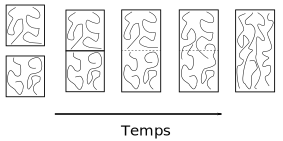
\includegraphics[scale=1]{welding_chain_diffusion.pdf}
	\caption{Diffusion des chaînes de polymère durant le soudage}
	\label{fig:polymer_diffusion}
\end{figure}

La diffusion des chaînes de polymère aux interfaces des polymères est un phénomène documenté. 
Le temps nécessaire pour réparer une fissure a été défini comme étant le temps nécessaire pour que les molécules adjacentes à la fissure diffusent à mi-chemin \cite{Prager1981a}. 
Un paramètre clé pour évaluer la vitesse du phénomène est le temps de reptation. 
Pour les polymères amorphes, on peut citer les travaux de Wool \cite{Wool1983,Wool1989} durant les années 1980. 
Ses travaux se sont concentrés sur l'évolution des propriétés mécaniques durant la phase de transition vers la diffusion complète des chaînes de polymère en condition isotherme. 
Il dénote entre autres que l'énergie nécessaire pour séparer des interfaces est une fonction de 4 paramètres : \begin{inparaenum}[(1)]
	\item le temps
	\item la température
	\item la pression
	\item la masse moléculaire. 
\end{inparaenum}
Ce dernier paramètre étant directement lié au temps de reptation tel que : 

\begin{equation}
T_r \approx M^3
\end{equation}

Lors de la diffusion des chaines de polymère dans les soudures en condition non isotherme, d'autres mécanismes entrent en jeu. 
Avant même que la diffusion des chaînes ne puisse prendre place, les faces en contact doivent atteindre un état de contact intime. 
Selon les modèles \cite{Yang2002}, le temps pour atteindre le contact intime est assez court et diminue très rapidement avec une hausse de la température et de la pression. 
Sans considération à cette première étape, à partir de données expérimentales en isotherme qui ont permis d'évaluer les temps de reptation en fonction de la température, pour des jonctions entre du PEI et du PEEK, Bastien \cite{Bastien1991} a développé des modèles pour prévoir la résistance obtenue après un soudage en condition non isotherme. 
Les résultats obtenus ont des marges d'erreur d'environ 20\%, mais confirment la possibilité d'obtenir des soudages de qualité avec des temps de mise en forme courts. 
Un modèle subséquent \cite{F.Yang2002} est parvenu à améliorer ces prédictions pour les conditions de variations rapides de température et permet d'évaluer le degré de guérison d'une interface avec plus de précision. 

\begin{figure}[]
	\centering
	\tikzset{
	basic/.style  = {draw, text width=6cm, drop shadow, rectangle},
	root/.style   = {basic, rounded corners=2pt, thin, align=center,
                   fill=gray!30},
	level 2/.style = {basic, rounded corners=5.5pt, thin,align=center, fill=gray!10,
                   text width=8em},
	level 3/.style = {basic, thin, align=left, fill=white, text width=6.em}
}


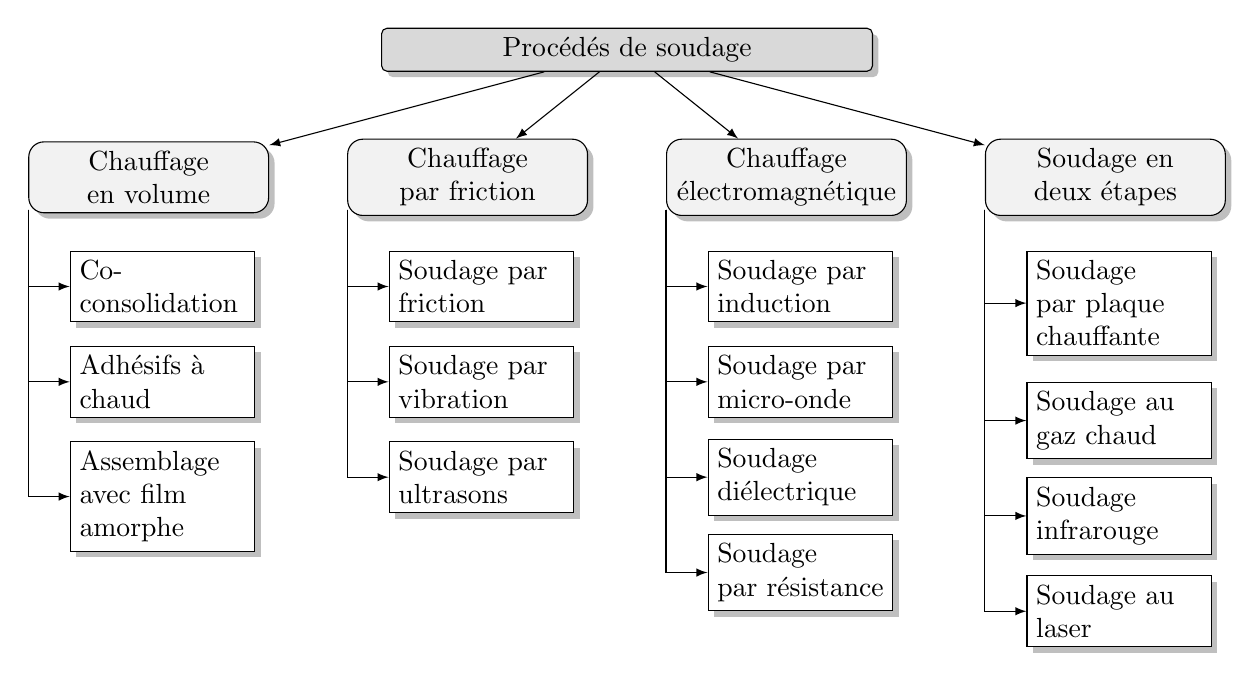
\begin{tikzpicture}[
	level 1/.style={sibling distance=45mm},
	edge from parent/.style={->,draw},
	>=latex,
	scale=0.9,
	level distance=1.8cm]

% root of the the initial tree, level 1
\node[root] {Procédés de soudage}
% The first level, as children of the initial tree
	child {node[level 2] (c1) {Chauffage en volume}}
	child {node[level 2] (c2) {Chauffage par friction}}
	child {node[level 2] (c3) {Chauffage électromagnétique}}
	child {node[level 2] (c4) {Soudage en deux étapes}};

% The second level, relatively positioned nodes
\begin{scope}[every node/.style={level 3}]
\node [below of = c1, xshift=5pt, yshift=-11pt] (c11) {Co-consolidation};
\node [below of = c11, yshift=-6pt] (c12) {Adhésifs à chaud};
\node [below of = c12, yshift=-13pt] (c13) {Assemblage avec film \mbox{amorphe}};

\node [below of = c2, xshift=5pt, yshift=-11pt] (c21) {Soudage par friction};
\node [below of = c21, yshift=-6pt] (c22) {Soudage par vibration};
\node [below of = c22, yshift=-6pt] (c23) {Soudage par ultrasons};

\node [below of = c3, xshift=5pt, yshift=-11pt] (c31) {Soudage par induction};
\node [below of = c31, yshift=-6pt] (c32) {Soudage par micro-onde};
\node [below of = c32, yshift=-6pt] (c33) {Soudage \mbox{diélectrique}};
\node [below of = c33, yshift=-6pt] (c34) {Soudage \mbox{par résistance}};

\node [below of = c4, xshift=5pt, yshift=-17pt] (c41) {Soudage par plaque \mbox{chauffante}};
\node [below of = c41, yshift=-14pt] (c42) {Soudage au gaz chaud};
\node [below of = c42, yshift=-6pt] (c43) {Soudage \mbox{infrarouge}};
\node [below of = c43, yshift=-6pt] (c44) {Soudage au laser};
\end{scope}

% lines from each level 1 node to every one of its "children"
\foreach \value in {1,2,3}
	\draw[->] (c1.195) |- (c1\value.west);

\foreach \value in {1,...,3}
	\draw[->] (c2.195) |- (c2\value.west);

\foreach \value in {1,...,4}
	\draw[->] (c3.195) |- (c3\value.west);

\foreach \value in {1,...,4}
	\draw[->] (c4.195) |- (c4\value.west);
\end{tikzpicture}

	\caption{Procédés de soudage (adapté de \cite{Ageorges2001a})}
	\label{fig:arbre_procédé_soudage}
\end{figure}

De nombreux procédés existent pour souder les polymères. 
La source de chaleur employée est généralement l'élément différenciateur entre les procédés (Fig. \ref{fig:arbre_procédé_soudage}). 
Il existe les procédés de chauffe en volume où les composants de l'assemblage sont chauffés en totalité. 
Ces procédés peuvent être réalisés entre autres dans un autoclave ou une presse chauffante. 
Un exemple de méthode soudage dans cette catégorie est le procédé Thermabond \cite{Smiley1991a}. 
En raison de leur grande demande énergétique, ces procédés sont généralement considérés comme étant peu efficaces. 
Une seconde famille de procédés produit un chauffage par friction, vibration \cite{Bates2007d} ou ultrason. 
À l'aide d'un mouvement alternatif rapide, la friction entre les composants produit un échauffement local. 
Ce même effet peut également être obtenu à l'aide d'ultrason en raison de l'hystérésis thermomécanique des matériaux. 
Ces méthodes pour joindre des composants sont rapides, mais peuvent induire un déplacement des fibres. 
Également, malgré ses très bonnes performances mécaniques \cite{Villegas2016}, l'application du soudage par ultrason est complexe pour les jonctions continues sur de longues distances en raison de sa nature point par point et de l'interaction entre les soudures successives \cite{Zhao2018}. 
Une autre famille de procédés regroupe les méthodes où le processus de soudage se produit en deux étapes distinctes. 
Dans un premier temps, les faces à joindre sont chauffées à l'aide de plaques chauffantes, de laser, d'infrarouges ou encore de gaz chaud. 
En second lieu, les faces sont ensuite mises en contact pour obtenir la jonction. 
Finalement, on peut regrouper ensemble les procédés utilisant une source de chaleur électromagnétique. 
Dans cette famille, on retrouve le soudage par induction \cite{Rudolf2000a,Ahmed2006a,Farahani2018}, le soudage  par pertes diélectrique et par micro-ondes \cite{Wu2012,Bowler2006a,Menendez2010d} et finalement le soudage par résistance \cite{houghton1984bonding,Eveno1988,Taylor1991,McKnight1997}. 
Les procédés de chauffe par induction, pertes diélectriques ou micro-ondes sont basés sur l'utilisation d'un champ électromagnétique alternatif. 
La différence entre ces procédés réside dans la fréquence du champ employé en allant des centaines de \si{\kilo\hertz} en induction jusqu'au \si{\giga\hertz} pour le chauffage par micro-ondes. 
Finalement, le soudage par résistance utilise les pertes par résistance dans un conducteur électrique pour obtenir un chauffage local à l'aide de l'effet de Joule. 
Le reste des travaux présentés dans cette thèse porteront sur le soudage par résistance. 

\begin{figure}[t]
	\centering
	\usetikzlibrary{arrows,shapes,positioning,shadows,trees}
\usetikzlibrary{decorations.pathmorphing} % Pour obtenir des lignes de coupes aléatoires
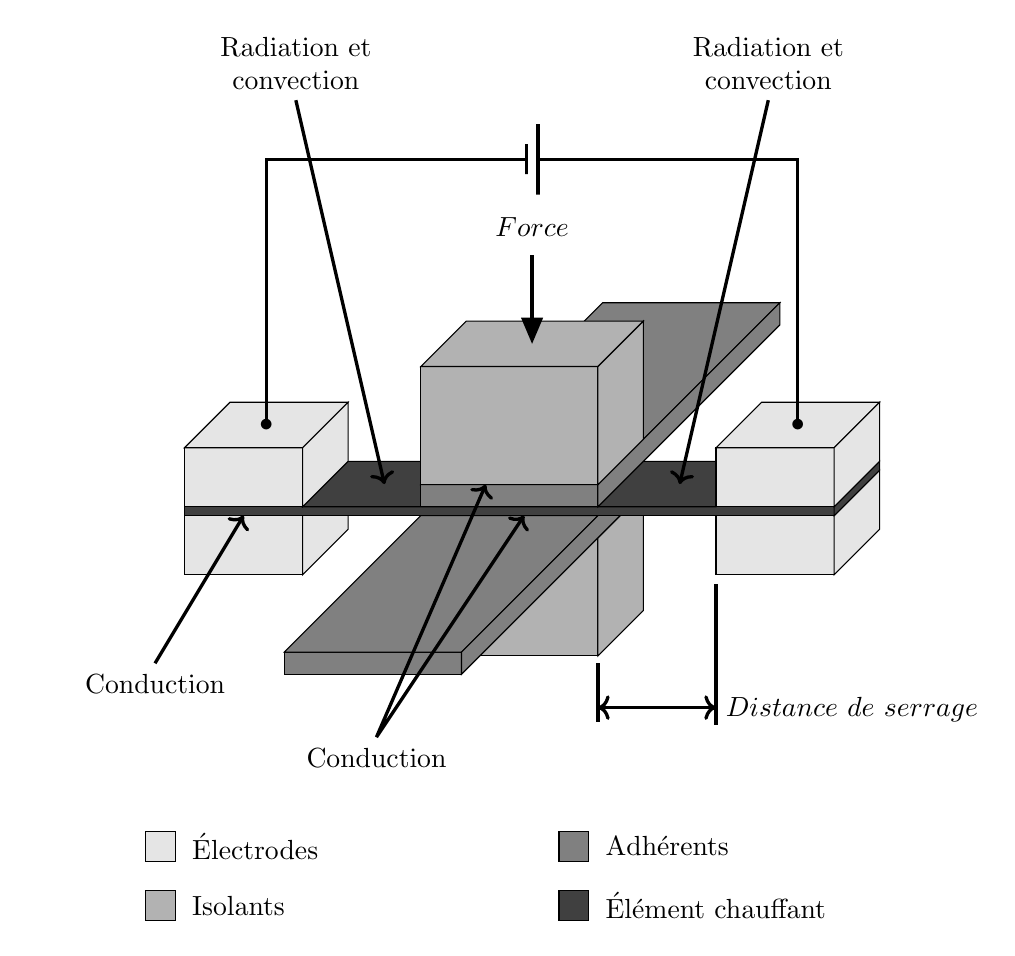
\begin{tikzpicture}[scale=0.75]


%Dimentions du bloc de connection
\def \largconnection{2}
\def \profconnection{2}
\def \hconnection{1.}

%Distance entre les deux blocs
\def \distance_connection{9}

%Épaisseur de l'élément résistif
\def \tele{0.15}

%Distance entre les blocs de connection et l'isolant
\def \gap{2}

%Dimensions des adhérent
\def \lcomp{6}
\def \tcomp{0.375}

%Épaisseur de l'isolant
\def \tbloc{2}

%Position et taille des annotations
\def \hsource{1.25*\profconnection}
\def \hpression{0.75*\profconnection}
\def \legende{0.5}
\def \distcotation{0.125}

%Couleurs
\def \colinsulator{blue!50}
\def \coladherend{green!50}
\def \colconnector{orange!60}
\def \colresistive{gray!50}

\def \colinsulator{black!30}
\def \coladherend{black!50}
\def \colconnector{black!10}
\def \colresistive{black!75}

%Bloc de pression inferieur
\draw[black,fill=\colinsulator] (\largconnection+\gap,-\tcomp-\tele-\tbloc,0) -- ++(0,\tbloc,0) -- ++(\distance_connection-\gap-\gap-\largconnection,0,0) -- ++(0,-\tbloc,0) -- cycle; %Face du devant
\draw[black,fill=\colinsulator] (\distance_connection-\gap,-\tcomp-\tele-\tbloc,0) -- ++(0,\tbloc,0) -- ++(0,0,-\profconnection) -- ++(0,-\tbloc,0) -- cycle; %Face de droite

%Adherant inferieur
\draw[black,fill=\coladherend] (\largconnection+\gap,-\tele-\tcomp,\lcomp) -- ++(0,\tcomp,0) -- ++(\distance_connection-\gap-\gap-\largconnection,0,0) -- ++(0,-\tcomp,0) -- cycle; %Face du devant
\draw[black,fill=\coladherend] (\largconnection+\gap,-\tele,\lcomp) -- ++(0,0,-\lcomp) -- ++(\distance_connection-\gap-\gap-\largconnection,0,0) -- ++(0,0,\lcomp) -- cycle; %Face du dessus
\draw[black,fill=\coladherend] (\distance_connection-\gap,-\tele,\lcomp) -- ++(0,-\tcomp,0) -- ++(0,0,-\lcomp-\profconnection) -- ++(0,\tcomp,0) -- cycle; %Face de droite

%Connection gauche inferieur
\draw[black, fill=\colconnector] (0,-\tele-\hconnection,0)--++(\largconnection,0,0)--++(0,\hconnection,0)--++(-\largconnection,0,0)--cycle; %Face du devant
\draw[black, fill=\colconnector] (\largconnection,-\tele-\hconnection,0)--++(0,\hconnection,0)-- ++(0,0,-\profconnection)--++(0,-\hconnection,0)--cycle; %Face de droite

%Connection droite inferieur
\draw[black, fill=\colconnector] (\distance_connection,-\tele-\hconnection,0)--++(\largconnection,0,0)--++(0,\hconnection,0)--++(-\largconnection,0,0)--cycle; %Face du devant
\draw[black, fill=\colconnector] (\largconnection+\distance_connection,-\tele-\hconnection,0)--++(0,\hconnection,0)--++(0,0,-\profconnection)--++(0,-\hconnection,0)--cycle; %Face de droite

%Element chauffant
\draw[black,fill=\colresistive] (0,0,0) -- (\largconnection+\distance_connection,0,0) -- ++(0,-\tele,0) -- (0,-\tele,0) -- cycle; %Face du devant
\draw[black,fill=\colresistive] (\largconnection,0,0) -- ++(0,0,-\profconnection) -- (\distance_connection,0,-\profconnection) -- (\distance_connection,0,0) -- cycle; %Face du dessus
\draw[black,fill=\colresistive] (\distance_connection+\largconnection,0,0) -- ++(0,0,-\profconnection) -- ++(0,-\tele,0) -- ++(0,0,\profconnection) -- cycle; %Face de droite

%Adherant superieur
\draw[black,fill=\coladherend] (\largconnection+\gap,0,0) -- ++(0,\tcomp,0) -- ++(\distance_connection-\gap-\gap-\largconnection,0,0) -- ++(0,-\tcomp,0) -- cycle; %Face du devant
\draw[black,fill=\coladherend] (\largconnection+\gap,\tcomp,0) -- ++(0,0,-\lcomp-\profconnection) -- ++(\distance_connection-\gap-\gap-\largconnection,0,0) -- ++(0,0,\lcomp+\profconnection) -- cycle; %Face du dessus
\draw[black,fill=\coladherend] (\distance_connection-\gap,\tcomp,0) -- ++(0,-\tcomp,0) -- ++(0,0,-\lcomp-\profconnection) -- ++(0,\tcomp,0) -- cycle; %Face de droite

%Connection gauche superieure
\draw[black, fill=\colconnector] (0,0,0)--(\largconnection,0,0)--++(0,\hconnection,0)--(0,\hconnection,0)--cycle; %Face du devant
\draw[black, fill=\colconnector] (0,\hconnection,0)--++(\largconnection,0,0)--++(0,0,-\profconnection)--++(-\largconnection,0,0)--cycle; %Face du dessus
\draw[black, fill=\colconnector] (\largconnection,0,0)--++(0,\hconnection,0)-- ++(0,0,-\profconnection)--++(0,-\hconnection,0)--cycle; %Face de droite

%Connection droite superieure
\draw[black, fill=\colconnector] (\distance_connection,0,0)--++(\largconnection,0,0)--++(0,\hconnection,0)--++(-\largconnection,0,0)--cycle; %Face du devant
\draw[black, fill=\colconnector] (\distance_connection,\hconnection,0)--++(\largconnection,0,0)--++(0,0,-\profconnection)--++(-\largconnection,0,-0)--cycle; %Face du dessus
\draw[black, fill=\colconnector] (\largconnection+\distance_connection,0,0)--++(0,\hconnection,0)--++(0,0,-\profconnection)--++(0,-\hconnection,0)--cycle; %Face de droite

%Bloc de pression superieur
\draw[black,fill=\colinsulator] (\largconnection+\gap,\tcomp,0) -- ++(0,\tbloc,0) -- ++(\distance_connection-\gap-\gap-\largconnection,0,0) -- ++(0,-\tbloc,0) -- cycle; %Face du devant
\draw[black,fill=\colinsulator] (\largconnection+\gap,\tcomp+\tbloc,0) -- ++(0,0,-\profconnection) -- ++(\distance_connection-\gap-\gap-\largconnection,0,0) -- ++(0,0,\profconnection) -- cycle; %Face du dessus
\draw[black,fill=\colinsulator] (\distance_connection-\gap,\tcomp,0) -- ++(0,\tbloc,0) -- ++(0,0,-\profconnection) -- ++(0,-\tbloc,0) -- cycle; %Face de droite

%Connection de la source de puissance
\draw [very thick] (0.5*\largconnection,\hconnection,-0.5*\profconnection) -- ++(0,\hsource+\tbloc,0) -- ++(0.5*\distance_connection-0.1,0,0) -- ++(0,-0.25,0) -- ++(0,0.5,0);
\draw [very thick] (0.5*\largconnection+\distance_connection,\hconnection,-0.5*\profconnection) -- ++(0,\hsource+\tbloc,0) -- ++ (-0.5*\distance_connection+0.1,0,0) -- ++(0,-0.6,0) -- ++ (0,1.2,0);
\draw (0.5*\largconnection,\hconnection,-0.5*\profconnection) node {$\bullet$} ;
\draw (0.5*\largconnection+\distance_connection,\hconnection,-0.5*\profconnection) node {$\bullet$} ;

%Pression
\draw [very thick, -triangle 45] (0.5*\largconnection+0.5*\distance_connection,\tbloc+\tcomp+\hpression,-0.5*\profconnection) -> ++(0,-\hpression,0);
\draw (0.5*\largconnection+0.5*\distance_connection,\tbloc+\tcomp+\hpression+0.15,-0.5*\profconnection) node[above] {$Force$};

%Clamping distance
\draw [very thick, black] (\distance_connection-\gap,-\tcomp-\tele-\tbloc-\distcotation,0) -- ++(0,-1,0);
\draw [very thick, black] (\distance_connection,-0.5*\tcomp-\hconnection-\distcotation,0) -- ++(0,-1-\tbloc+\hconnection-\tcomp,0);
\draw [very thick, black, <->] ((\distance_connection-\gap,-\tcomp-\tele-\tbloc-\distcotation-0.75,0) -- ++ (\gap,0,0);
\draw (\distance_connection,-0.5*\tcomp-\tcomp-\distcotation-\tbloc-.75,0) node[right] {$Distance \ de \ serrage$};

%Identification des modes de refroidissement
\draw [very thick,<-] (\largconnection+0.5*\gap,0,-0.5*\profconnection) -- ++(-1.5,6.5,0) node[above, text width=3cm, align=center] {{Radiation et \\ convection}};
\draw [very thick,<-]  (\distance_connection-0.5*\gap,0,-0.5*\profconnection) -- ++(1.5,6.5,0) node[above, text width=3cm, align=center] {{Radiation et \\ convection}};
\draw [very thick,<-]  (0.5*\largconnection,-\tele,0) -- ++(-1.5,-2.5,0) node[below, text width=3cm, align=center] {{Conduction}};
\draw [very thick,<->]  (0.5*\distance_connection+0.625*\gap,-\tele,0) -- ++(-2.5,-3.75,0) node[below, text width=3cm, align=center] {{Conduction}} --(0.5*\distance_connection+0.3*\gap,\tcomp,0) ;


%Legende
\begin{scope}[yshift=-11.cm, xshift=-5.5cm]

	\begin{scope}[xshift=-7cm]
		\draw [black, fill=\colconnector] (\distance_connection+1.42*\profconnection,2.5*\tbloc) rectangle ++(\legende,\legende);
		\draw (\distance_connection+1.42*\profconnection+1.25*\legende,2.5*\tbloc+0.5*\legende) node[right]{Électrodes} ;

		\draw [black, fill=\colinsulator] (\distance_connection+1.42*\profconnection,2.5*\tbloc-2*\legende) rectangle ++(\legende,\legende);
		\draw (\distance_connection+1.42*\profconnection+1.25*\legende,2.5*\tbloc-1.5*\legende) node[right]{Isolants} ;
	\end{scope}

	\draw [black, fill=\coladherend] (\distance_connection+1.42*\profconnection,2.5*\tbloc) rectangle ++(\legende,\legende);
	\draw (\distance_connection+1.42*\profconnection+1.25*\legende,2.5*\tbloc+0.5*\legende) node[right]{Adhérents} ;

	\draw [black, fill=\colresistive] (\distance_connection+1.42*\profconnection,2.5*\tbloc-2*\legende) rectangle ++(\legende,\legende);
	\draw (\distance_connection+1.42*\profconnection+1.25*\legende,2.5*\tbloc-1.5*\legende) node[right]{Élément chauffant} ;
\end{scope}
\end{tikzpicture}

	\caption{Schéma du procédé de soudage par résistance avec identification des modes de conduction de chaleur}
	\label{fig:schema_soudage_resistance}
\end{figure}

Lors du soudage par résistance, un élément chauffant poreux est positionné entre les adhérents (Fig. \ref{fig:schema_soudage_resistance}). 
Généralement, des blocs isolants sont positionnés autour de la soudure pour réduire les pertes thermiques. 
Des électrodes sont fixées aux deux extrémités de l'élément chauffant à une distance variable du bord des adhérents nommée «distance de serrage». 
Avant d'injecter un courant dans le système et tout au long du procédé de soudage, une force est appliquée sur la zone à souder. 
Après un temps prédéterminé, la source électrique est arrêtée tout en maintenant la pression sur la soudure pendant le refroidissement. 
Une fois que la soudure est refroidie en dessous de la température de transition vitreuse des polymères, il est possible de retirer du montage l'assemblage obtenu. 
Il est à noter que l'élément chauffant reste captif de la soudure à la fin du procédé. 
La possibilité de produire des soudures continues en soudage par résistance a également été démontrée en laboratoire \cite{Shi2015a}. 
Les équations de contact intime et d'autohesion par diffusion des chaînes en situation de soudage non isotherme ont été appliquées par Ageorges \cite{Ageorges1998} et Colak \cite{Colak2002} afin d'approximer théoriquement des fenêtres d'opération. 

Si on fixe la géométrie du montage de soudage et le choix des matériaux, les principaux paramètres ayant une influence sur la qualité du joint sont 
\begin{inparaenum}[(1)]
	\item la puissance électrique
	\item le temps de soudage
	\item les effets de bords et les modes de conduction de chaleur
	\item la pression appliquée sur la soudure. 
\end{inparaenum}
Globalement, il faut également tenir compte des propriétés des matériaux employés ainsi que la géométrie des composants du montage. 

\begin{figure}[]
	\centering
	\includegraphics[scale=0.85]{process_window}
	\caption{Fenêtre de puissance pour le procédé de soudage (tiré de \cite{Hou2001})}
	\label{fig:process_window}
\end{figure}

Afin d'optimiser la qualité de la soudure, la puissance électrique et le temps de soudage peuvent facilement être modifiés. 
La plage de puissance ainsi que l'énergie nécessaire (produit de la puissance et du temps) à la production d'une soudure satisfaisante sont documentées dans la littérature \cite{Hou1999a}. 
Des puissances surfaciques allant de 80 à \SI{150}{\kilo\watt\per\square\metre} permettent de produire des soudures satisfaisantes. 
D'autres auteurs ont également utilisé des puissances allant jusqu'à \SI{282}{\kilo\watt\per\square\metre} \cite{Dube2007} avec des temps plus courts. 
Certains auteurs utilisent également de très fortes puissances pulsées de l'ordre de \SI{600}{\kilo\watt\per\square\metre} avec un temps de repos de quelques secondes entre chaque pulsation afin d'obtenir une température plus uniforme dans la zone soudée et réduire la quantité d'énergie requise  \cite{Arias1996}. 
La figure \ref{fig:process_window} présente une fenêtre de puissance de soudage en fonction du temps afin d'obtenir un soudage entre des pièces composites avec un élément chauffant en acier inoxydable ou en composite de fibre de carbone avec une matrice en PEI. 
Ce graphique présente également des courbes d'énergie équivalente. 
On peut obtenir l'énergie produite en multipliant la puissance au temps d'application selon l'équation : 

\begin{equation}
E = P \times t
\end{equation}

Où $E$ est la quantité d'énergie en Joules, $P$ est la puissance en Watts et $t$ est le temps en secondes. 
On peut obtenir la puissance d'un élément chauffant de section constante, en fonction de ses propriétés électriques et de ses dimensions à l'aide des équations suivantes. Dans ces équations, $V$ est la tension en volts, $I$ est l'intensité du courant en ampères, $R$ est la résistance en $\ohm$, $L$ est la longueur en mètres du conducteur, $A_s$ est l'aire de la section du conducteur en mètres carrés et $\rho_{ele}$ est résistivité en $\ohm \cdot$mètres. 

\begin{equation}
P = V \times I
\end{equation}

\begin{equation}
P = R \times I^2
\end{equation}

\begin{equation}
P = \frac{\rho_{ele} \times L}{A_s} \ I^2
\end{equation}

\begin{equation}
P = \frac{V^2}{\rho_{ele}} \ \frac{A_s}{L}
\end{equation}

Il est possible de lier la résistivité ($\rho_{ele}$) d'un matériau à sa conductivité ($\sigma$, $\kappa$ ou $\gamma$ selon les auteurs) en Siemens par mètres à l'aide de l'équation suivante. 

\begin{equation}
\sigma = \frac{1}{\rho_{ele}}
\end{equation}

Dans le cas des éléments pour le soudage résistif, ces équations sont simplifiées sous la forme suivante. Où $l$ est la largeur en mètre du grillage et $\gamma$ est la résistivité spécifique en $\ohm$. 

\begin{equation}
R = \gamma \ \frac{L}{l}
\label{EQ:resistance_element_chauffant}
\end{equation}

Pour utiliser l'équation \ref{EQ:resistance_element_chauffant}, il est nécessaire de caractériser au préalable l'élément chauffant afin de connaître sa résistance spécifique. 
Cette dernière équation pose également l'hypothèse d'un élément de composition relativement homogène. 
Les effets des dimensions des mailles ainsi que le diamètre des fils ont été étudiés dans la littérature et il a été trouvé que le ratio entre le ratio d'aire ouverte et le diamètre du fil est un critère important pour le soudage avec un grillage métallique \cite{Dube2012a}. 

Pour ce qui est des effets de bords et des modes de conduction de chaleur, cet effet est principalement dépendant de la géométrie du montage et de la nature des matériaux. 
Cependant, pour un montage de soudage donné, un contrôle limité de ce paramètre est parfois possible en modifiant la distance de serrage des électrodes. 
Comme indiqué à la figure \ref{fig:schema_soudage_resistance}, les pertes thermiques de l'élément chauffant changent de mode de diffusion en fonction de leur position dans la soudure. 
Dans les zones où l'élément chauffant est positionné entre les adhérents composites ou lorsqu'il est en contact avec les électrodes, la diffusion thermique se produit principalement par conduction. 
Dans les zones où l'élément chauffant est exposé (entre les bords des adhérents et les électrodes), les pertes thermiques se produisent plutôt par radiation et convection naturelle. 
Puisque ces derniers modes de conduction de chaleur sont moins efficaces, un certain contrôle de la température au bord du laminé est possible en ajustant la distance de serrage \cite{Talbot2013}. 
Il est impossible d'éliminer totalement ces effets de bord, mais il est possible de viser des paramètres de soudage qui en réduisent l'effet. 

En ce qui concerne la pression appliquée sur la soudure, plusieurs chercheurs ont présenté l'impact de la pression sur la qualité des soudures obtenues. 
En premier lieu, pour les soudures de laminés avec une matrice en polyétherimide (PEI), Ageorges \cite{Ageorges2000a} a observé des signes de déconsolidation des laminés lorsqu'une faible pression, de l'ordre de \SI{0.1}{\mega\pascal}, est employée.
Il a aussi noté le déplacement des fibres et un trop grand écoulement causé par la compression du laminé lorsqu'une pression supérieure à \SI{1.6}{\mega\pascal} est employée. 
Il définit au final une plage entre 0.2 et \SI{1.6}{\mega\pascal} comme cible. 
Une autre étude plus détaillée \cite{Shi2017} a observé l'effet de la pression sur la formation de porosités et la déconsolidation pour des laminés de fibres de verre et PEI. 
Les résultats ont démontré qu'une pression d'au moins \SI{0.8}{\mega\pascal} est nécessaire pour éliminer les porosités à l'interface causées par l'humidité et la déconsolidation du laminé. 

\begin{figure}[h]
	\centering
	\usetikzlibrary{arrows,shapes,positioning,shadows,trees,arrows.meta}
\usetikzlibrary{decorations.pathmorphing} % Pour obtenir des lignes de coupes aléatoires
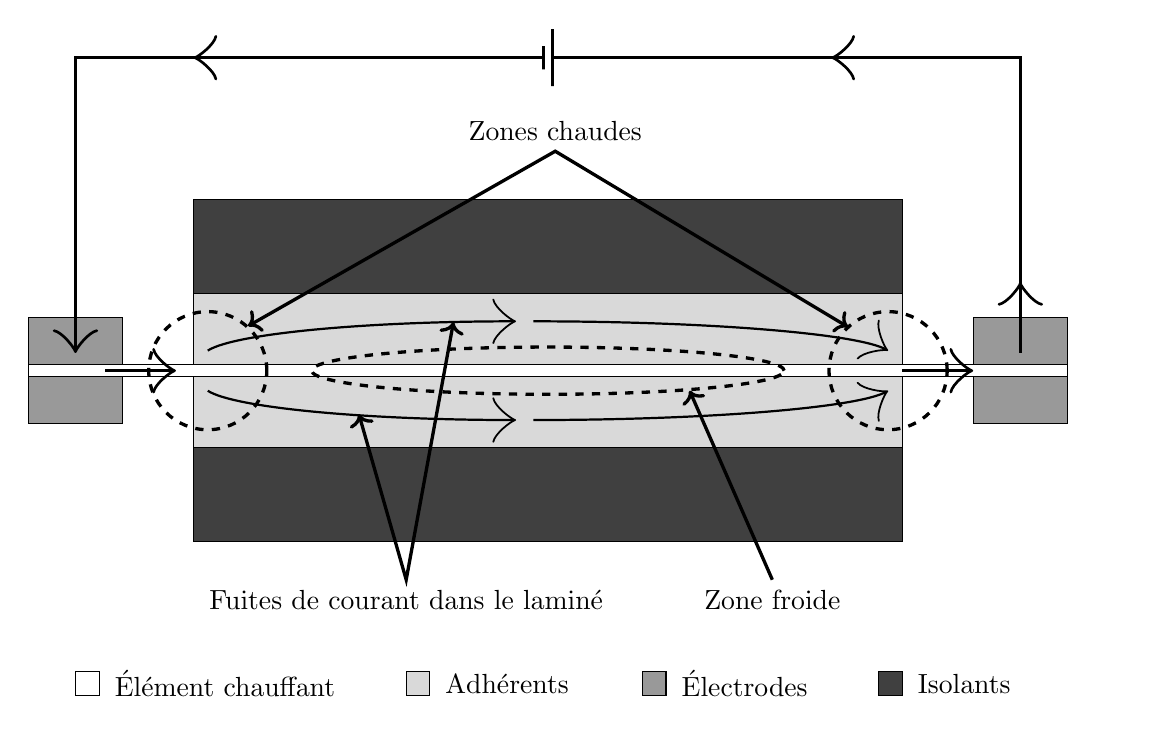
\begin{tikzpicture}[scale=0.6]


%Dimentions du bloc de connection
\def \largconnection{2}
\def \hconnection{1.}

%Distance entre les deux blocs
\def \distance_connection{20}

%Épaisseur de l'élément résistif
\def \tele{0.25}

%Distance entre les blocs de connection et l'isolant
\def \gap{1.5}

%Dimensions des adhérent
\def \tcomp{1.5}

%Épaisseur de l'isolant
\def \tbloc{2}

%Position et taille des annotations
\def \hsource{3.5}
\def \legende{0.5}
\def \distcotation{0.125}

%Couleurs
\def \colinsulator{blue!50}
\def \coladherend{green!50}
\def \colconnector{orange!60}
\def \colresistive{gray!50}

\def \colinsulator{black!75}
\def \coladherend{black!15}
\def \colconnector{black!40}
\def \colresistive{black!0}

%Bloc de pression inferieur
\draw[black,fill=\colinsulator] (\largconnection+\gap,-\tcomp-\tele-\tbloc) -- ++(0,\tbloc) -- ++(\distance_connection-\gap-\gap-\largconnection,0) -- ++(0,-\tbloc) -- cycle; %Face du devant

%Adherant inferieur
\draw[black,fill=\coladherend] (\largconnection+\gap,-\tele-\tcomp) -- ++(0,\tcomp) -- ++(\distance_connection-\gap-\gap-\largconnection,0) -- ++(0,-\tcomp) -- cycle; %Face du devant

%Connection gauche inferieur
\draw[black, fill=\colconnector] (0,-\tele-\hconnection)--++(\largconnection,0)--++(0,\hconnection)--++(-\largconnection,0)--cycle; %Face du devant


%Connection droite inferieur
\draw[black, fill=\colconnector] (\distance_connection,-\tele-\hconnection,0)--++(\largconnection,0,0)--++(0,\hconnection,0)--++(-\largconnection,0,0)--cycle; %Face du devant


%Element chauffant
\draw[black,fill=\colresistive] (0,0,0) -- (\largconnection+\distance_connection,0,0) -- ++(0,-\tele,0) -- (0,-\tele,0) -- cycle; %Face du devant


%Adherant superieur
\draw[black,fill=\coladherend] (\largconnection+\gap,0,0) -- ++(0,\tcomp,0) -- ++(\distance_connection-\gap-\gap-\largconnection,0,0) -- ++(0,-\tcomp,0) -- cycle; %Face du devant


%Connection gauche superieure
\draw[black, fill=\colconnector] (0,0,0)--(\largconnection,0,0)--++(0,\hconnection,0)--(0,\hconnection,0)--cycle; %Face du devant

%Connection droite superieure
\draw[black, fill=\colconnector] (\distance_connection,0,0)--++(\largconnection,0,0)--++(0,\hconnection,0)--++(-\largconnection,0,0)--cycle; %Face du devant

%Bloc de pression superieur
\draw[black,fill=\colinsulator] (\largconnection+\gap,\tcomp,0) -- ++(0,\tbloc,0) -- ++(\distance_connection-\gap-\gap-\largconnection,0,0) -- ++(0,-\tbloc,0) -- cycle; %Face du devant


%Connection de la source de puissance
\draw [very thick] (0.5*\largconnection,\hconnection) -- ++(0,\hsource+\tbloc) -- ++(0.5*\distance_connection-0.1,0) -- ++(0,-0.25) -- ++(0,0.5);
\draw [very thick] (0.5*\largconnection+\distance_connection,\hconnection) -- ++(0,\hsource+\tbloc) -- ++ (-0.5*\distance_connection+0.1,0) -- ++(0,-0.6) -- ++ (0,1.2);


%Courant dans le laminé
\draw[thick, -{Classical TikZ Rightarrow[length=3mm]} ] (\largconnection+1.2*\gap,0.2*\tcomp) arc (170 : 90 : {0.5*\distance_connection-2.25*\gap} and 0.75);
\draw[thick, -{Classical TikZ Rightarrow[length=3mm]} ] (\largconnection+1.2*\gap,-0.2*\tcomp-\tele) arc (-10 : -90 : -{0.5*\distance_connection+2.25*\gap} and 0.75);
\draw [thick, {Classical TikZ Rightarrow[length=3mm]}- ] (\distance_connection-1.2*\gap,0.2*\tcomp) arc (10 : 90 : {0.25*\distance_connection+1.75*\gap} and 0.75);
\draw [thick, {Classical TikZ Rightarrow[length=3mm]}- ] (\distance_connection-1.2*\gap,-0.2*\tcomp-\tele) arc (-10 : -90 : {0.25*\distance_connection+1.75*\gap} and 0.75);
\draw [very thick, {Classical TikZ Rightarrow[length=3mm]}- ] (0.5*\largconnection,0.25*\hconnection) -- ++(0,1.5);
\draw [very thick, -{Classical TikZ Rightarrow[length=3mm]}] (0.5*\largconnection+\distance_connection,0.25*\hconnection) -- ++(0,1.5);
\draw [very thick, -{Classical TikZ Rightarrow[length=3mm]}] (\largconnection-0.25*\gap,-0.5*\tele) -- ++(1*\gap,0);
\draw [very thick, -{Classical TikZ Rightarrow[length=3mm]}] (\distance_connection-1*\gap,-0.5*\tele) -- ++(1.*\gap,0);
\draw [very thick, -{Classical TikZ Rightarrow[length=3mm]}] (\distance_connection-1*\gap,\hconnection+\hsource+\tbloc) -- ++(-\gap,0);
\draw [very thick, -{Classical TikZ Rightarrow[length=3mm]}] (\largconnection+2*\gap,\hconnection+\hsource+\tbloc) -- ++(-1.*\gap,0);

%Identification des fuites de courant
\draw [very thick,<->]  (0.35*\distance_connection,-\tele-0.8) -- ++(1,-3.5) node[below, text width=9cm, align=center] {{Fuites de courant dans le laminé}} --(0.45*\distance_connection,\tcomp-0.6) ;

% zones chaudes
\begin{scope}[radius=1.25, very thick, dashed]
\draw (\largconnection+\gap+0.3,-0.5*\tele) circle ;
\draw (-\gap+\distance_connection-0.3,-0.5*\tele) circle ;
\end{scope}
\draw [very thick,<->]  (\largconnection+\gap+1.155,0.82) -- ++(6.5,3.7) node[above, text width=9cm, align=center] {{Zones chaudes}} --(-\gap+\distance_connection-1.15,\tcomp-0.7) ;

% zone froide
\draw [very thick, dashed] (0.5*\distance_connection+0.5*\largconnection,-0.5*\tele) ellipse [x radius=5,y radius=0.5] ;
\draw [very thick,<-]  (0.7*\distance_connection,-\tele-0.3) -- ++(1.75,-4) node[below, text width=9cm, align=center] {{Zone froide}} ;

%Legende
\begin{scope}[yshift=-12.cm, xshift=1cm]

\begin{scope}[xshift=12cm]
\draw [black, fill=\colconnector] (0,2.5*\tbloc) rectangle ++(\legende,\legende);
\draw (1.25*\legende,2.5*\tbloc+0.5*\legende) node[right]{Électrodes} ;
\end{scope}

\begin{scope}[xshift=7cm]
\draw [black, fill=\coladherend] (0,2.5*\tbloc) rectangle ++(\legende,\legende);
\draw (1.25*\legende,2.5*\tbloc+0.5*\legende) node[right]{Adhérents} ;
\end{scope}

\begin{scope}[xshift=0cm]
\draw [black, fill=\colresistive] (0,2.5*\tbloc) rectangle ++(\legende,\legende);
\draw (1.25*\legende,2.5*\tbloc+0.5*\legende) node[right]{Élément chauffant} ;
\end{scope}

\begin{scope}[xshift=17cm]
\draw [black, fill=\colinsulator] (0,2.5*\tbloc) rectangle ++(\legende,\legende);
\draw (1.25*\legende,2.5*\tbloc+0.5*\legende) node[right]{Isolants} ;
\end{scope}

\end{scope}
\end{tikzpicture}

	\caption{Schéma du phénomène de fuite de courant}
	\label{fig:schema_fuite_de_courant}
\end{figure}

Un phénomène à surveiller lors du soudage résistif est la fuite de courant dans le corps des laminés de fibres de carbone. 
Ce phénomène peut se produire lorsque les bords de l'élément chauffant entrent en contact électrique avec les fibres de carbone du laminé et forment un circuit électrique parallèle à l'élément résistif \cite{Hou1999a,Ageorges2000}. 
Ce nouveau circuit réduit le chauffage de la zone soudée, peut empêcher la soudure au centre du joint et peut dégrader le polymère aux bords \cite{Dube2008}. 
On observe alors des zones chaudes aux bords des laminés et une zone froide au centre (Fig. \ref{fig:schema_fuite_de_courant}). 
Plusieurs approches existent pour éliminer ce problème. 
Il est possible d'ajouter une couche de fibre de verre isolante entre l'élément chauffant et le laminé \cite{Hou1999a}. 
Cette solution a le désavantage d'ajouter un élément étranger dans la zone soudée et d'augmenter l'épaisseur des joints. 
Il est également possible d'isoler le grillage métallique à l'aide d'un revêtement isolant \cite{Dube2008,Dube2009a}. 
Ce revêtement empêche tout contact électrique entre les fibres et l'élément chauffant. 
Finalement, il est également possible d'employer une couche d'un polymère possédant une température de mise en forme inférieure à la température de fonte du polymère de base \cite{Stavrov2005a}. 

Le soudage par résistances des composites thermoplastique est généralement réalisé avec un élément chauffant en acier inoxydable ou encore en fibre de carbone. 
Initialement, il était naturel pour les chercheurs d'utiliser en élément chauffant en composites à fibre de carbone \cite{Ageorges2000a,houghton1984bonding,Eveno1988}. 
Cependant, des problèmes persistants étaient causés par la connexion électrique avec les fibres, le manque de répétabilité dans les résultats obtenus et la mise à l'échelle \cite{McKnight1997}. 
Le passage à des éléments chauffants en acier inoxydable a permis d'améliorer grandement la répétabilité du procédé ainsi que sa capacité à être mis à l'échelle \cite{Hou1999a}.  
Cependant, dans certaines circonstances, le manque d'adhésion entre les éléments chauffants en acier inoxydable et la matrice peut être le point faible d'une soudure par résistance \cite{Dube2007,Dube2012a,Dube2009a,Shi2014,Shi2015a}. 

\subsection{Soudage avec matériaux mixtes}

Les composites à matrice thermoplastiques peuvent également être joints à d'autres matériaux. 
Plusieurs chercheurs travaillent au soudage entre des adhérents thermoplastiques et métalliques. 
Les méthodes employées varient du soudage au point par friction \cite{Goushegir2016}, au soudage par ultrason \cite{Balle2009,Kruger2004} jusqu'à des combinaisons de soudage par laser avec un chauffage par induction \cite{Weidmann2018}. 
Ce dernier exemple est d'ailleurs intéressant par son approche où ils texturent d'abord l'adhérent métallique à l'aide d'un laser. 
Lors du soudage subséquent, le polymère vient remplir les porosités crées en surface pour obtenir un blocage mécanique entre les matériaux. 
Ce procédé a d'ailleurs fait l'objet d'une démonstration technologique visant à présenter une cellule de production automatisée pour des pièces du domaine automobile \cite{Gardiner2019a}. 

En plus des métaux, il est possible, dans certains cas de souder des adhérents en composites à matrice thermodurcissable. 
En employant une couche de polymère thermoplastique moulée avec le thermodurcissable lors de sa fabrication, des chercheurs ont pu souder des composites thermoplastiques avec des pièces en époxy \cite{Lionetto2018a,FernandezVillegas2015}

\section{Nanocomposites conducteurs}

Les nanocomposites sont définis par l'Office québécois de la langue française depuis 2005 comme : 

\begin{quote}
	Matériau qui comporte deux ou plusieurs phases distinctes dont une au moins intègre des éléments qui possèdent une dimension pouvant varier entre 1 et 100 nanomètres.
\end{quote}

Les nanocomposites sont constitués, au minimum, d'une matrice, souvent polymérique, et de particules de taille nanométriques. 
L'ajout de nanoparticules aux polymères permet de modifier leurs propriétés mécaniques \cite{Thostenson2002a}, électriques \cite{Zheng2003a}, optiques \cite{Hu2014} et thermiques \cite{Diez-Pascual2009, Al-Saleh2009c}. 
Les nanocomposites trouvent des applications dans plusieurs domaines \cite{Andrews2001, Thostenson2001c, Mittal2014h}. 

Les modifications des propriétés conférées par les nanoparticules sont dépendantes de leurs propriétés propres ainsi que de leur géométrie. 
Les propriétés exceptionnelles des nanoparticules proviennent en partie du ratio entre leur surface et leur volume. 
Elles exposent des surfaces spécifiques beaucoup plus importantes que tout autre matériau macroscopique. 

En raison de leur excellente conductivité électrique, les nanoparticules à base de carbone sont utilisées dans ce projet. 
Pour cette raison, la revue de l'état des connaissances se concentre sur cette famille de nanoparticules ainsi que sur leurs nanocomposites associés. 

\subsection{Nanotubes de carbone}

Découverts accidentellement en 1991 \cite{iijima1991}, les nanotubes de carbones se retrouvent maintenant dans presque tous les domaines de la science des matériaux et de nouvelles applications leur sont trouvés régulièrement. 
Les nanotubes de carbone sont composés d'une structure régulière de feuilles graphitiques de carbone enroulées et jointes pour former un ou des tubes concentriques qui peuvent être refermés aux extrémités par des structures sphériques, comme présenté à la figure \ref{structure_nanotube}. 

\begin{figure}[htb]
	\centering
	\includegraphics[width=0.7\textwidth]{Saito1992.pdf}
	\caption{Structure d'un nanotube de carbone (adapté de \cite{Saito1992}, avec permission)}
	\label{structure_nanotube}
\end{figure}

Un nanotube peut être constitué d'un seul tube ou d'une série de tubes emboîtés concentriquement. 
On différencie les nanotubes à simple paroi des nanotubes à parois multiples. 
Le comportement des nanotubes est fonction de l'angle d'hélice de la structure. 
Pour les nanotubes à simple paroi on peut obtenir des nanotubes aux propriétés métalliques jusqu'à semi-conductrice avec des variations de cet angle \cite{Saito1992}. 
Des traitements permettent de purifier les nanotubes et surtout de les séparer selon leur comportement \cite{Makama2013}. 
Généralement, pour les nanotubes multi parois, l'angle d'hélice est moins bien contrôlé et varie d'une couche à l'autre.
On obtient ainsi des nanotubes aux propriétés intermédiaires. 

Les nanotubes de carbone ont des conductivités électriques allant jusqu'à \SI{10e6}{\siemens\per\centi\metre}  \cite{Sathyanarayana2013} et thermiques de l'ordre de \SI{6600}{\watt\per\metre\per\kelvin} \cite{Berber2000}
Ces propriétés sont fortement dépendantes de l'orientation et la présence de défauts dans la structure cristalline des nanotubes. 
Les modules de Young rapportés pour les nanotubes de carbone multi parois sont aux alentours de 2 TPa avec des résistances à la traction entre 11 et \SI{63}{\giga\pascal} \cite{Mittal2014h}. 
Les propriétés des nanotubes de carbone en font d'excellents candidats pour la fabrication de nanocomposites.

Les nanotubes de carbone sont principalement produits par décharge d'arc, par ablation laser, par déposition chimique en phase vapeur \cite{Sathyanarayana2013} ou à l'aide de torches au plasma \cite{Kim2009e}. 
Les nanotubes produits peuvent présenter des défauts de cristallinité tels que la présence de pentagones et d'heptagones ou encore des absences dans la structure régulière d'hexagones. 
Ces défauts affectent les propriétés, mais peuvent également être utilisés pour introduire des fonctionnalisations de surface. 

%\subsection{Nanofibres de carbone}
%
%Les nanofibres de carbone partagent un bon nombre de similarité avec les nanotubes de carbone mais un coût beaucoup plus faible. 
%Ils sont produits par déposition chimique en phase vapeur tout comme les nanotubes de carbone. 
%Ils peuvent ensuite être graphitisés pour améliorer leur pureté et augmenter leur conductivité électrique \cite{Al-Saleh2009c}. 
%La principale différence entre les nanotube et les nanofibres se situe au niveau de leur morphologie. 
%Les nanofibres ont généralement une structure semblable à des bols empilés. 
%Ces bols peuvent être distincts ou liés ensemble en spirale \cite{Al-Saleh2009c}. 
%Cette structure est distincte des tubes circulaires qui composent les nanotubes. 
%Les propriétés des nanofibres sont également similaires à celles des nanotubes de carbone mais avec un niveau de conductivité électrique réduit. 
%
%\subsection{Graphène}
%
%Les nanoparticules de graphène possèdent la même structure hexagonale que les atomes de carbone des parois des nanotubes de carbone. 
%Cependant, au lieu de former un tube, les atomes forment des lamelles de l'épaisseur d'un seul atome de carbone. 

\subsection{Méthodes de production des nanocomposites}

Pour tirer profit à l'échelle macroscopique des propriétés des nanomatériaux, il est nécessaire de les mélanger dans une matrice. 
Plusieurs méthodes permettent d'obtenir des mélanges avec les polymères thermoplastiques. 

Une première méthode est la mise en solution des nanotubes \cite{Mohammad2006}.
Lors de cette procédure, les nanotubes sont mis en suspension métastable dans un solvant. 
Cette méthode est appropriée pour les polymères solubles, les polymères à très faible viscosité et pour les monomères \cite{Ma2010}. 
Pour obtenir une distribution homogène, il est nécessaire d'employer un générateur d'ultrason afin de séparer les agglomérats de nanoparticules. 
Des surfactants sont souvent utilisés pour stabiliser les dispersions de nanoparticules \cite{Huang2012}. 
Le brassage par bassin à ultrason est une des seules méthodes procurant la densité d'énergie nécessaire pour réduire les agglomérats de nanotubes à simple paroi, mais elle peut également induire des dommages et raccourcir les tubes \cite{Huang2012}. 
Cette méthode ne doit donc pas être employée sans considération des propriétés nécessaires pour l'application finale puisque la réduction de la longueur des tubes \cite{Grossiord2008a} et les traitements de surface \cite{Diez-Pascual2010, Ma2008} peuvent affecter les propriétés finales.  
Il est à noter que la densité énergétique nécessaire pour séparer les nanotubes multi parois est beaucoup plus faible et que d'autres méthodes peuvent les séparer sans induire autant de dommage à leur structure \cite{Huang2012}. 
Le mélange produit par la mise en solution peut être employé directement ou, si le solvant utilisé est compatible avec le polymère utilisé, il est possible d'obtenir un composite homogène en évaporant le solvant pour conserver les nanoparticules ainsi que le polymère. 

Une seconde méthode de production est le mélange à l'état fondu. 
Cette méthode est particulièrement applicable aux polymères thermoplastiques, la viscosité résiduelle du polymère induit des efforts de cisaillement avec une densité d'énergie suffisante pour réduire les agglomérats de nanotubes multi parois \cite{Huang2012}. 
Ce brassage peut s'effectuer avec un mélangeur mécanique ou à l'aide d'une d'extrudeuse. 
Ces deux techniques ont l'avantage de ne pas causer de dommages aux nanotubes. 

Une autre technique pouvant s'appliquer aux polymères thermoplastiques est le broyage par boulets. 
Ce processus utilise les chocs et le brassage des billes métalliques dans un contenant fermé en rotation pour réduire en poudre les polymères et ainsi que les agglomérats de nanotubes.
Cette technique endommage les nanotubes, mais il est possible d'y introduire des composés chimiques pour fonctionnaliser les nanotubes afin de modifier leurs propriétés \cite{Ma2010}. 

\begin{table}[]
	\centering
	\resizebox{\textwidth}{!}{%
		\begin{tabular}{@{}l p{1.2in} p{2.5in} p{2.75in} @{}}
			\toprule
			Techniques            & Facteurs                    &                                                                                        &                                                                                                     \\
			\cmidrule(l){2-4}     & Endommagement des nanotubes & Types de matrice compatibles                                                           & Principaux paramètres                                                                               \\ \midrule
			Ultrasonification     & Oui                         & Polymère soluble, polymère ou oligomère à faible viscosité, monomère                   & Puissance et mode d'ultrasonification, durée                                                        \\
			Broyage par boulets   & Oui                         & Granules et poudre (polymère ou monomère)                                              & Durée du broyage, vitesse de rotation, taille des boulets, ratio entre les boulets et les nanotubes \\
			Extrusion             & Non                         & Thermoplastiques                                                                       & Température, géométrie et vitesse de rotation de la vis                                             \\
			Mélange par agitation & Non                         & Thermoplastiques, polymère soluble, polymère ou oligomère à faible viscosité, monomère & Taille et géométrie de l'agitateur, vitesse de rotation, temps de mélange                           \\ \bottomrule
		\end{tabular}
	}
	\caption{Résumé des méthodes de mélange (adapté de \cite{Ma2010})}
	\label{methodes_de_melange}
\end{table}

Les solutions mentionnées précédemment visent à produire des nanocomposites à dispersion homogène dans l'ensemble de la structure. 
Il est également de produire des nanocomposites nanostructurés avec une ségrégation des nanocharges qui permet la création d'un réseau continu à une plus petite quantité de nanoparticules \cite{Al-Saleh2011, Li2015a, Deng2014a, Du2011a, Pang2014c, Jia2015}. 
Cette technique peut offrir des composites avec une conductivité électrique beaucoup plus élevée. 
Lors de la fusion de ces polymères, il est cependant possible qu'une diffusion des nanocharges se produise qui affectera drastiquement les propriétés électriques après le changement dans la nanostructure \cite{Wu2012}. 
Ce comportement pourrait d'ailleurs être utilisé comme méthode pour contrôler la puissance dégagée lors du soudage. 

Un des défis lors de la production des nanocomposites est de stabiliser la séparation des nanoparticules qui ont tendance à s’agglomérer.
Cette stabilité peut être atteinte en augmentant l'affinité des nanoparticules avec la matrice d'accueil ou par répulsion entre elles. 
Ces effets peuvent être obtenus par une fonctionnalisation de la surface des nanotubes \cite{Xie2005}. 
La fonctionnalisation peut affecter les propriétés macroscopiques des nanocomposites \cite{Ma2008}. 

\subsection{Conductivité électrique des nanocomposites}

L'ajout de nanoparticules conductrices permet de transformer des polymères non conducteurs en nanocomposites conduisant l'électricité. 
La modification des propriétés électriques est principalement une fonction de la quantité de nanoparticules dispersées, de leur nature, de la qualité de la dispersion, de la nature du polymère et des modifications de surface apportées aux nanoparticules. 

Les variations de la conductivité électrique observées ne peuvent pas être expliquées par la simple loi des mélanges. 
À partir d'une certaine concentration, les nanotubes de carbone forment un réseau continu dans la matrice. 
Cette concentration est nommée seuil de percolation.
En dessous du seuil de percolation, la conductivité du nanocomposite change peu et il reste isolant. 
Lorsque le réseau est initialement formé, la conductivité électrique du nanocomposite change totalement et une augmentation très rapide de la conductivité électrique, de l'ordre de plusieurs décades, peut être observée. 
Par la suite, la conductivité du nanocomposite continue d'augmenter avec l'ajout de nanoparticules, mais avec une pente beaucoup plus faible. 
L'évolution de la conductivité électrique d'un nanocomposite suit trois régimes distincts qui sont fonction de la concentration en nanocharges conductrices. 
La figure \ref{percolation_electrique} présente une courbe de conductivité électrique en fonction de la concentration en nanotubes de carbone multi parois dans une matrice de PEEK. 
Le facteur de forme \cite{Hu2008}, le niveau de dispersion, l'orientation des particules dans la matrice \cite{Xie2011c} et les traitements de surface sont des facteurs qui ont un impact direct sur le seuil de percolation. 

\begin{figure}[]
	\centering
	\fbox{
		\includegraphics[width=0.6\textwidth]{percolation_electrique.png}}
	\caption{Conductivité électrique d'un nanocomposite de PEEK et de nanotubes de carbone (tiré de \cite{Bangarusampath2009}, avec permission)}
	\label{percolation_electrique}
\end{figure}

La plupart des auteurs se concentrent sur la caractérisation du seuil de percolation et peu de mesures de conductivité sont disponibles pour des concentrations élevées de nanotubes. 
Les plus grands gains en conductivité électrique peuvent en effet être observés à ces concentrations et la réduction de la concentration en nanotubes permet de réduire les coûts du matériau. 
Les auteurs rapportent des seuils de percolation variant entre 0,0021\% à 15\% \cite{Bauhofer2009}. 
Une portion des résultats publiés sont résumés à la figure \ref{percolation_articles}. 

\begin{figure}[]
	\centering
	\fbox{
		\includegraphics{percolation_litterature.pdf}}
	\caption{Seuil de percolation minimal reporté et nombre d'articles publiés pour certains systèmes nanocomposites (tiré de \cite{Bauhofer2009}, avec permission)}
	\label{percolation_articles}
\end{figure}

En ce qui concerne les concentrations plus élevées de nanoparticules conductrices, quelques articles peuvent être soulignés. 
Par exemple, une conductivité de \SI{10 000}{\siemens\per\metre} a été atteinte avec une matrice de PMMA et une concentration de 10\% de nanotubes à simple paroi \cite{Bauhofer2009}. 
Cependant, malgré quelques rares résultats exceptionnels, l'ensemble des données publiées présente une très grande variabilité, car un grand nombre de facteurs varient entre chaque étude.
Il n'existe aucune courbe maître pouvant permettre de généraliser tous ces résultats. 
Le consensus est qu'une bonne dispersion favorise la conductivité électrique \cite{Bauhofer2009} et que les principaux paramètres gouvernant la conductivité sont 
\begin{inparaenum}
	\item le facteur de forme des nanotubes
	\item une bonne dispersion des agglomérats de nanotubes à l'échelle nanométrique
	\item une distribution uniforme des nanotubes ou des agglomérats à l'échelle microscopique   
\end{inparaenum} \cite{Li2007a}.

Également, une fois le seuil de percolation franchi, les conductivités obtenues augmentent moins rapidement que pourrait le suggérer la loi des mélanges. 
Certains travaux \cite{Untereker2009,Cauchy2018} en sont venus à la conclusion que la conductivité électrique obtenue lors du mélange d'une matrice chargée en micro ou nano matériaux est limitée par la résistance de contact élevée entre les particules. 
La dépendance envers la résistance de contact a également rapporté par d'autres auteurs \cite{Li2007a}. 

La fonctionnalisation des nanotubes est généralement employée pour faciliter leur dispersion, mais elle peut également affecter les propriétés électriques du nanocomposite. 
Certaines modifications vont entraîner une chute de a conductivité électrique tandis que d'autres vont permettre de réduire la résistance de contact. 

Cette variation des effets des divers types de fonctionnalisation par rapport à la conductivité électrique est documentée dans la littérature scientifique. 
Par exemple, il a été démontré que la fonctionnalisation avec des groupes carboxyliques (COOH) produit une réduction très importante de la conductivité \cite{Guadagno2011}. 
Dans cette dernière étude, même en quadruplant la quantité de nanotubes de carbone, les nanotubes fonctionnalisés présentaient une conductivité électrique encore inférieure aux nanotubes non traités. 
La fonctionnalisation avec des groupements amines (NH$_2$) produit également une réduction de la conductivité électrique \cite{Ma2008} et il est postulé que cette réduction est en partie du à la dégradation de la structure des nanotubes nécessaire au dépôt des groupes fonctionnels qui réduit la conductivité des nanotubes sans réduire la résistance de contact \cite{Pandey2012a}.
Même dans le cas de particules métalliques, l'ajout d'une fonctionnalisation à base du composé organique 
1-Octanethiol a causé une baisse de la conductivité électrique \cite{Gelves2008a}. 
Au contraire, le dépôt de particules d'argent a pour effet de permettre une réduction de la résistance de contact et ainsi augmente la conductivité électrique  \cite{Ma2010,Cauchy2017}

Les méthodes de fonctionnalisation par enroulement de polymère produisent généralement une réduction de la conductivité électrique \cite{Diez-Pascual2010, Huang2012}. 
Un auteur a cependant obtenu une hausse de la conductivité lorsqu'il a utilisé du polyaniline (PANI), un polymère conducteur, comme agent de revêtement des nanotubes \cite{Vankayala2011}. 
En utilisant un polymère conducteur compatible avec les nanotubes et avec la matrice de nylon 6, l'auteur a pu réduire la résistance de contact tout en améliorant la dispersion des charges. 

\FloatBarrier
\section{Élastomères thermoplastiques}  

Un second concept clé pour la réalisation d'une jonction flexible est en lien avec la nature des élastomères thermoplastiques. 
Les élastomères en général sont une famille de polymère dont la plage de température d'utilisation se situe au-dessus de la température de transition vitreuse. 
Au-delà de celle-ci, les polymères entrent en phase caoutchoutique et les chaînes de peuvent commencer à se déplacer et glisser les unes par rapport aux autres. 

\begin{figure}[h]
	\centering
	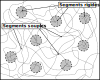
\includegraphics[scale=1]{structure_tribloc.pdf}
	\caption{Exemple de structure pour un élastomère thermoplastique triblocs}
	\label{fig:structure_tribloc}
\end{figure}

Les élastomères commerciaux sont souvent obtenus par une réticulation partielle entre les chaînes de polymère, appelé vulcanisation dans le cas de la transformation du  caoutchouc naturel, ayant pour but de bloquer une partie de la mobilité des chaînes sans pour autant leur retirer leur flexibilité. 
Les élastomères thermoplastiques obtiennent quant à eux ce comportement à l'aide de leur structure et de leur composition. 
Par l'emploi de segments de nature différente, on obtient une structure où les terminaisons composées de segments rigides viennent se lier pour former des blocs à l'intérieur de la structure du matériau \cite{Holden1969}. 
En raison de la faible miscibilité entre les deux polymères causé par une incompatibilité thermodynamique, on observe une ségrégation entre les différentes phases. 
Les blocs rigides, composés de polymère qui sont utilisés sous leur température de transition rigide, procurent le même effet que la réticulation entre les chaînes composées, dans leur portion centrale, d'un second polymère utilisé au-dessus de sa température de transition vitreuse \cite{Holden2002}. 
Les blocs rigides sont également capables de fondre une fois chauffé et on peut ainsi remettre en forme l'élastomère. 
Les élastomères thermoplastiques ont généralement des structures copolymères en triblocs ou multi blocs. 
Les élastomères copolymères triblocs ont des segments rigides aux deux extrémités. 
Ces dernières sont connectées au travers d'un réseau biphasique dans la structure de l'élastomère (Fig. \ref{fig:structure_tribloc}). 
Contrairement aux élastomères triblocs, figés aux deux extrémités, les élastomères multi blocs utilisent l'enchevêtrement et l'interaction entre les chaînes souples et rigides pour maintenir leur intégrité. 
La présence de segments de polymère semi-cristallins au travers d'une chaîne amorphe permet aux segments cristallins de se lier pour bloquer l'écoulement de la structure (Fig. \ref{fig:structure_TPECryst}). 
Alternativement, dans certains cas, les segments cristallins peuvent également être des segments de polymère amorphe \cite{Holden2002}. 

\begin{figure}[h]
	\centering
	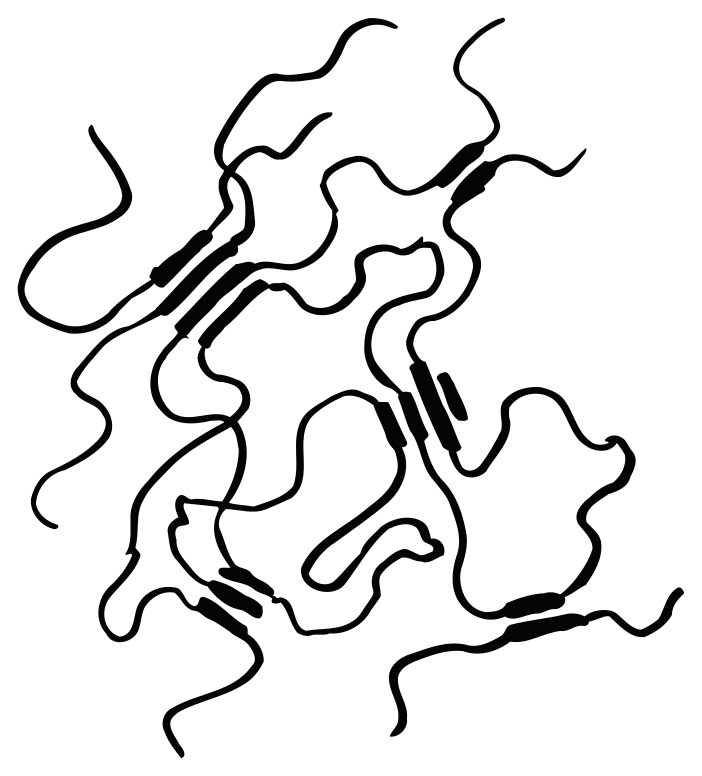
\includegraphics[scale=0.3]{CrystTPE_CC0.pdf}
	\caption{Exemple de structure pour un élastomère thermoplastique avec segments cristallins [licence CC0]}
	\label{fig:structure_TPECryst}
\end{figure}

En ce qui concerne la soudure des élastomères, très peu de références peuvent être trouvées à ce propos et encore moins en ce qui concerne le soudage entre des matériaux mixtes \cite{Chan2016,Hollande1998}. 
Aucun article trouvé ne traitait du soudage où se produisait une diffusion des chaînes dans un autre polymère thermoplastique. 